
\subsection{Résultats en test}

Pour comparer nos différents modèles, nous avons utilisé deux mesures: la précision et la \emph{Mean Average Precision} sur trois prédictions (MAP@3).
Le choix de cette deuxième mesure est le fait que c'est cette mesure qui est utilisée pour évaluer les modèles dans le projet Kaggle \footnote{\url{https://www.kaggle.com/c/quickdraw-doodle-recognition}} présenté par \emph{Google AI}.
Cette mesure calcule la précision, mais donne des points partiels de 0.5 et 0.33 pour les cas où le modèle prédit la vraie classe en deuxième ou troisième position.

Voici la liste des résultats obtenus sur le jeu de données de test qui comporte 340 000 (1000 par classe) données:

\begin{center}
\setlength{\tabcolsep}{2mm}
\begin{tabular}{c c c}
\toprule
\textbf{Modèle} & \textbf{Accuracy} & \textbf{MAP@3}  \\

\midrule

\textit{Resnet18} & 77.57&83.78 \\
\textit{Resnet18} données ciblés  &79.58&85.42 \\
Ensemble avec classif  & 75.92 &82.64       \\
Ensemble avec moyenne     & \textbf{79.93}&\textbf{85.66}        \\



\bottomrule
\addlinespace[3mm]
\end{tabular}
\end{center}

On peut voir que l'échantillonnage ciblé du second modèle nous apporte un gain de précision d'environ 2\% (de 77.57\% à 79.58\% en précision et de 83.78\% à 85.42\% en MAP@3). 
C'est un résultat assez intéressant puisque cette technique n'est pas standard, mais apporte tout de même un gain de performance non négligeable. 
On peut supposer que cela a permis de gagner un peu en précision sur les classes moins bien prédites sans trop affecter celles qui étaient déjà bien classées.
On peut expliquer cela par le fait que les classes les plus difficiles à prédire sont celles qui ont une grande variabilité dans les dessins faits par les utilisateurs. 
Il faut donc plus d'exemples différents de cette classe pour bien capter toutes leurs particularités alors qu'on n'a besoin que de quelques observations pour les classes plus simples.


Malheureusement, la modèle par ensemble avec la couche de classification supplémentaire ne donne pas les résultats escomptés.
Avec une précision en test de 75.92\%, c'est le plus faible de tous les modèles essayés. On pense toutefois que si on avait eu un entraînement qui converge, ce modèle aurait donné des performances au moins aussi bonnes que le pire des deux modèles \emph{ResNet18}.


Le meilleur d'entre tous est le modèle qui fait une moyenne simple des deux premiers modèles avec une précision de 79.93\% et une MAP@3 de 85.66\% en test.

Ces résultats sont loins des meilleurs modèles qui ont été soumis pour la compétition Kaggle où les meilleurs compétiteurs ont obtenus des MAP@3 d'environ 95\%, mais nous sommes tout de même satisfaits des résultats obtenus compte tenu des ressources de calcul limitées qui étaient à notre disposition.
Également, on peut expliquer une bonne partie de cette différence de performance par le fait que notre modèle n'utilise pas l'information temporelle des vecteurs de dessins. 
Certaines équipes ont utilisé des modèles aussi simples que nous, mais ont utilisés plusieurs canaux d'image pour représenter l'évolution temporelle du dessin et ont pu obtenir très rapidement des MAP@3 supérieurs à 90\%.


\subsection{Analyse d'erreur}
Il est intéressant de regarder quelques prédictions de notre modèle pour mieux comprendre où sont les erreurs qu'il commet. 
On peut également observer la précision par classe en test pour voir quelles classes fonctionnent moins bien.


Voici un tableau de quelques classes avec une accuracy assez faible (modèle avec échantillons ciblés):
\begin{center}
\begin{tabular}{|c|c|}
\hline
\textbf{Classe} & \textbf{Accuracy} \\ \hline
tornado & 0.142 \\ \hline
birthday cake & 0.254 \\ \hline
guitar & 0.492 \\ \hline
pool & 0.558 \\ \hline
trombone & 0.640 \\ \hline
frog & 0.693 \\ \hline
\end{tabular}
\end{center}



On constate que la plupart de ces classes de dessin ne sont évidentes à dessiner et plusieurs techniques peuvent être utilisées pour faire certains de ses dessins. 
Un humain peut généralement reconnaître le dessin d'un même objet, même si celui est représenté de plusieurs manières différentes (ex: grenouille à la figure \ref{frogs}). 
Ce n'est toutefois pas aussi évident pour réseau de convolution.

Pour aller chercher une précision supplémentaire sur ces classes problématiques, nous aurions pu construire des classificateurs binaires spécialisés pour ces classes et les utiliser dans notre modèle par ensemble.

On peut observer des classes ayant bien performées: 

\begin{center}
\begin{tabular}{|c|c|}
\hline
\textbf{Classe} & \textbf{Accuracy} \\ \hline
snowman & 0.953 \\ \hline
star & 0.951 \\ \hline
ladder & 0.951 \\ \hline
envelope & 0.946 \\ \hline
rainbow & 0.931 \\ \hline
clock & 0.924 \\ \hline
\end{tabular}
\end{center}


On constate qu'il s'agit principalement de classes qui sont simples et rapides à dessiner au complet et il n'existe pas plusieurs façons possibles pour dessiner ces dessins
Par exemple \emph{snowman}, \emph{star} et \emph{ladder} sont souvent dessinés de la même façon.


On peut également observer quelques mauvaises prédictions de notre modèle sur la figure \ref{comborate}

\begin{figure}[h]
	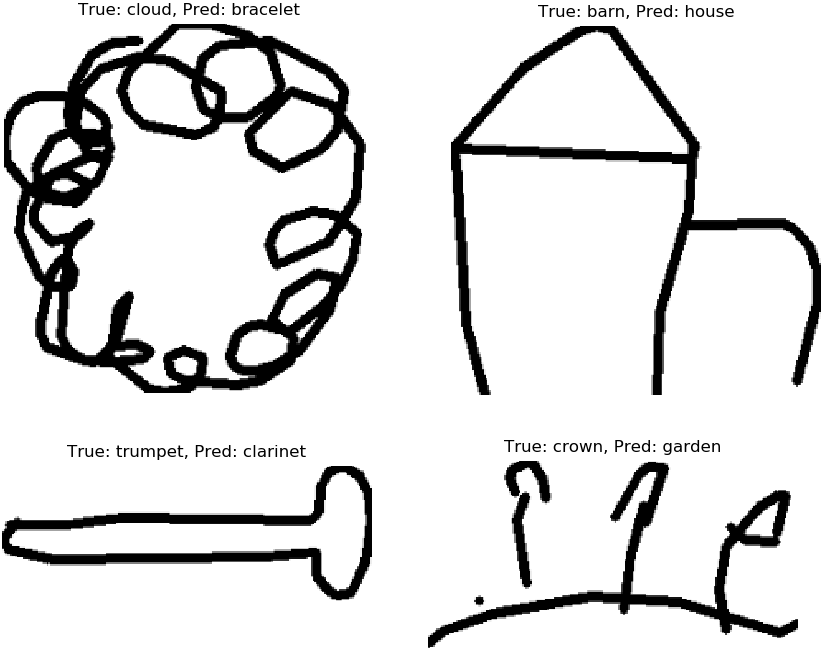
\includegraphics[width=\linewidth]{images/combo_rate.png} % Figure image
	\caption{Images mal prédites} % Figure caption
	\label{comborate} 
\end{figure}

On peut voir que même quand le modèle se trompe, ses prédictions sont quand mêmes représentatives de ce qu'un humain pourrait voir.
Par exemple, même si la première image est supposée être un nuage, on pourrait interpréter ce dessin comme étant un bracelet.


Même si sa précision n'est pas si élevée, le modèle nous donne quand même l'impression de performer assez bien étant donné que la plupart de ses prédictions font souvent du sens pour un humain même si elles ne sont pas parfaites.
Il est possible de tester l'application créée dans le cadre de ce projet en clonant le projet Github du projet\footcite{Github:repo} pour tester d'autres exemples du prédiction du modèle.
